% -*- TeX -*-
\documentclass[aspectratio=169]{beamer}
\usepackage[none]{hyphenat}
\usepackage{tikz}
\usepackage{annotate-equations}
\usepackage{natbib}


\usepackage{mathtools} % equations

\title{Bayesian Inference: Very Short Intro}
\author{Matt Knepley\\
Brad Aagaard}
\institute{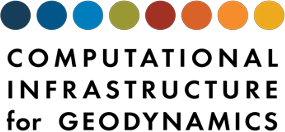
\includegraphics[scale=1.5]{../../logos/cig_logo_dots}%
  \hspace{4em}%
\raisebox{1em}{\includegraphics[scale=1.0]{../../logos/cig_short_pylith}}}
\date{June 11, 2026}


% ---------------------------------------------------- CUSTOMIZATION
\usetheme{CIG}
\input{../style}

% --------------------------------------------------------- DOCUMENT
\begin{document}

% ------------------------------------------------------------ SLIDE
\maketitle
\logo{\includegraphics[height=4.5ex]{../../logos/cig_short_pylith}}


% ========================================================== SECTION
\section{Introduction}


% ------------------------------------------------------------ SLIDE
\begin{frame}
  \frametitle{Uncertainty Quantification}

  \begin{itemize}
  \item What is the uncertainty in my observations?
  \item How accurate is my model?
    \begin{itemize}
    \item What is the accuracy of my solver?
    \item What is the accuracy (discretization error) of my mesh+discretization?
    \item How well do I know my input parameters?
    \end{itemize}
  \item What is the uncertainty in my inversion?
    \begin{itemize}
    \item How big is the null space?
    \end{itemize}
  \end{itemize}
\end{frame}



% ========================================================== SECTION
\section{Bayesian Inference}

% ------------------------------------------------------------ SLIDE
\begin{frame}

  \Large\begin{center}
    Bayesian Inference
    \vfill
    Matt Knepley

  \end{center}
\end{frame}

% ------------------------------------------------------------ SLIDE
\begin{frame}

  \Large\begin{center}
  \Huge Never believe anything\\

  \bigskip
  \bigskip

  \qquad until you run it.
\end{center}
\end{frame}


% ------------------------------------------------------------ SLIDE
\begin{frame}{Bayesian Inference}
\Huge
\qquad Using data to improve\\

\bigskip
\bigskip

\qquad\qquad an approximate distribution
\end{frame}


% ------------------------------------------------------------ SLIDE
\begin{frame}{Bayes' Rule}\Huge
\begin{align*}
  P(H | D) = \frac{P(D | H) P(H)}{P(D)}
\end{align*}
\end{frame}


% ------------------------------------------------------------ SLIDE
\begin{frame}{Bayes' Rule}\Huge
\begin{align*}
  P(H | D) = \frac{P(D | H) P(H)}{\sum_i P(D | H_i) P(H_i)}
\end{align*}
\end{frame}


% ------------------------------------------------------------ SLIDE
\tikzset{annotate equations/text/.style={font=\normalsize}}
\begin{frame}{Bayes' Rule}\Huge
\begin{align*}
  \eqnmark[blue]{posterior}{\underbrace{P(H | D)}} = \eqnmark[cyan]{likelihood}{\overbrace{\frac{P(D | H)}{\sum_i P(D | H_i) P(H_i)}}} \eqnmark[red]{prior}{\underbrace{P(H)}}
  \annotate[yshift=-1em]{below}{posterior}{posterior}
  \annotate[yshift=1em]{above}{likelihood}{likelihood}
  \annotate[yshift=-1em]{below}{prior}{prior}
\end{align*}
\end{frame}


% ------------------------------------------------------------ SLIDE
\begin{frame}{Strategy 1: Lots of Samples}\Huge
\begin{center}
  \href{https://academic.oup.com/gji/article/202/2/1289/593030}{\citep{baumannkaus2015}}
\end{center}

\bigskip

\begin{itemize}\LARGE
  \item[] Fit entire posterior
  \medskip
  \item[] Combine brute-force sampling with MCMC
  \medskip
  \item[] Likelihood samples can be very expensive
\end{itemize}
\end{frame}


% ------------------------------------------------------------ SLIDE
\begin{frame}{Strategy 1: Lots of Samples}\Huge
\begin{center}
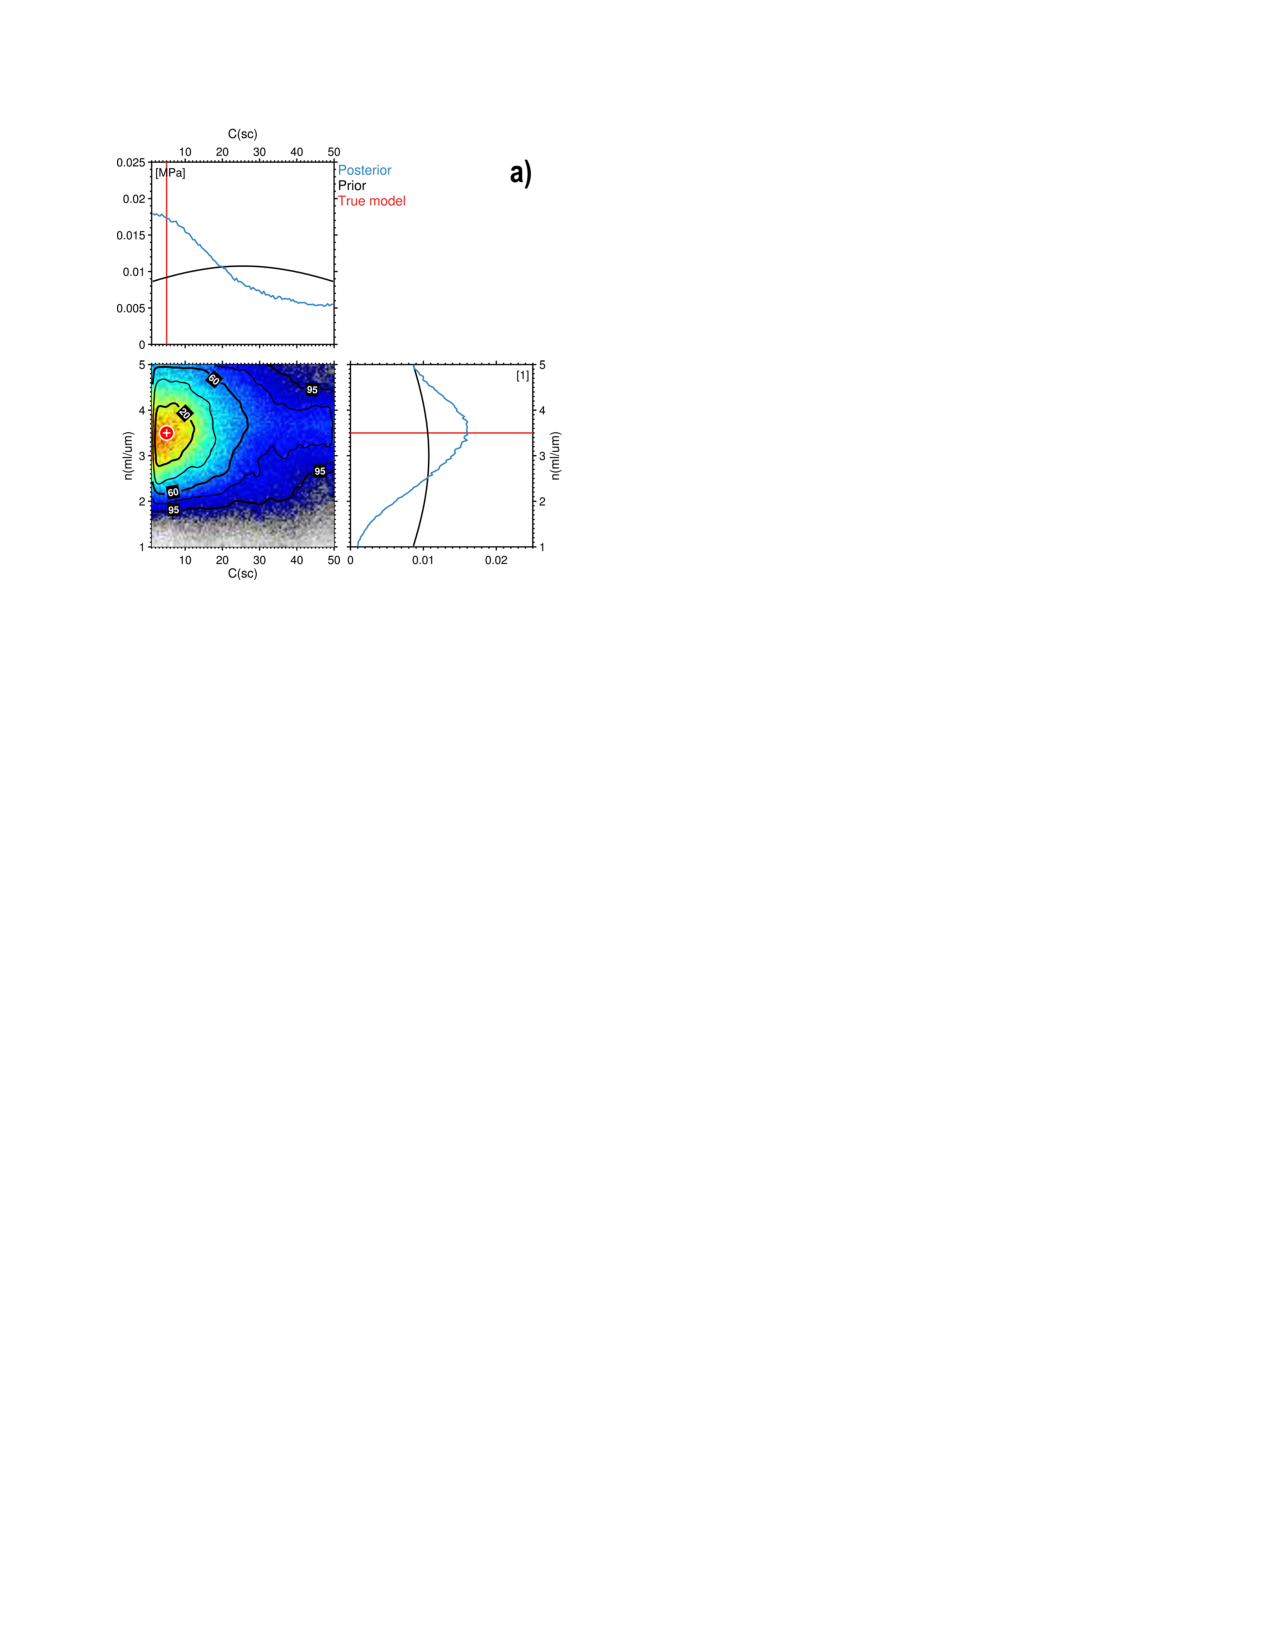
\includegraphics[height=0.8\textheight]{figures/Bayesian/BayesMCMCKaus}\\
\small Baumann and Kaus, 2015
\end{center}
\end{frame}


% ------------------------------------------------------------ SLIDE
\begin{frame}{Strategy 2: Lots of Approximations}\Huge
\begin{center}
  \href{https://arxiv.org/pdf/1407.1517}{\citep{buithanhgirolami2014}}
\end{center}

\bigskip

\begin{itemize}\LARGE
  \item[] Approx. posterior around the maximum (MAP) point
  \medskip
  \item[] Sample with MCMC
  \medskip
  \item[] Solve adjoint to get gradient of cost function
  \medskip
  \item[] Low-rank Hessian approximation
\end{itemize}
\end{frame}


% ------------------------------------------------------------ SLIDE
\begin{frame}{Cross-Fade}\Huge
\begin{center}
  \href{https://academic.oup.com/gji/article/239/3/1629/7783283}{\citep{minson2024}}
\end{center}

\bigskip

\begin{itemize}\LARGE
  \item[] Continuation method in distributions
  \medskip
  \item[] Does not require likelihood evaluations
  \medskip
  \item[] Calculates marginal likelihood for design optimization
\end{itemize}
\end{frame}


% ------------------------------------------------------------ SLIDE
\begin{frame}[allowframebreaks]{References}
  \bibliographystyle{chicagoAA}
    {\scriptsize\bibliography{presentations}}
\end{frame}


% ------------------------------------------------------------ SLIDE
\begin{frame}
  \frametitle{Discussion}

  \begin{itemize}
  \item What are the obstacles for quantifying uncertainty in your work?
  \item What techniques are available for quantifying uncertainty?
  \item What resources (e.g., software) are available?
  \end{itemize}
\end{frame}


% ======================================================================
\end{document}


% End of file
